\documentclass[11pt]{article}
\usepackage{geometry}
\geometry{letterpaper, margin=1in}
\usepackage{times}
\usepackage{graphicx}
\usepackage{amsmath}
\usepackage{booktabs}
\usepackage{hyperref}
\usepackage{subcaption}
\usepackage{float}
\usepackage{listings}
\usepackage{xcolor}

\title{Bridging Vision and Language: An Empirical Study on Continuous Connectors and Discrete VQ-VAE Architectures}
\author{Programming Assignment 3: Implementation and Analysis Report}
\date{\today}

\begin{document}

\maketitle

\begin{abstract}
This comprehensive report details the implementation, exhaustive evaluation, and profound analytical insights derived from the Vision-Language Models (VLMs) programming assignment (PA3). We explore two fundamentally orthogonal paradigms for multimodal alignment. In Part A, we investigate Continuous Connector VLMs, utilizing a frozen CLIP vision encoder whose semantic patches are mathematically rotated into the continuous embedding space of an autoregressive language model (SmolLM2-360M) via a Multi-Layer Perceptron (MLP). Through empirical plotting, we highlight the critical role of language replay in preventing catastrophic forgetting and provide a deep geometrical analysis of the Modality Gap across training phases. In Part B, we pivot to Discrete VQ-VAEs, training a convolutional vector quantizer from scratch to compress synthetic images into a discrete codebook. We demonstrate how carefully expanding the vocabulary via an overlay technique, combined with sequential multi-objective optimization, allows the language model to act symmetrically as both a visual reasoning engine and an autoregressive image generator. This report integrates directly generated experimental plots to establish insights into alignment geometries, memory constraints, and the trade-offs between continuous semantics and discrete tokenization.
\end{abstract}

\section{Introduction}

The integration of visual reasoning into Large Language Models (LLMs) represents one of the most dynamic frontiers in artificial intelligence. However, a structural divide exists: language models are discrete autoregressive sequence processors, while images are high-dimensional continuous grids. This assignment tackles this divide by implementing and testing two contrasting architectures.

\textbf{Part A} focuses on the continuous projection paradigm. A frozen Contrastive Language-Image Pretraining (CLIP) encoder extracts continuous semantic visual patches. A connector network learns to project these continuous representations into the LLM's continuous embedding space.
\textbf{Part B} explores the discrete tokenization paradigm. A Vector Quantized Variational Autoencoder (VQ-VAE) compresses visual inputs into a discrete, finite codebook. These codebook indices are appended directly to the LLM's vocabulary.

\section{Part A: Continuous Connector VLMs}

In Part A, we bridge OpenAI's \texttt{clip-vit-base-patch32} with HuggingFace's \texttt{SmolLM2-360M-Instruct}. 

\subsection{Methodology and Architecture Setup}

\subsubsection{Data Pipeline and Caching}
We utilized a stratified subset of CIFAR-10 (1000 images per class for training). To mitigate severe computational bottlenecks, we adopted a feature caching strategy. Images were preprocessed using the exact `CLIPImageProcessor` normalization standards. The images were passed through the frozen CLIP vision transformer, explicitly discarding the `CLS` token to retain the 49 spatial patches ($[49, 768]$). We generated five distinct VQA templates per image to test different reasoning axes: Recognition, Binary logic, Abstraction, Attribute detection, and Category grouping.

\subsubsection{Phase 1: Connector Initialization}
Feeding untrained continuous visual embeddings into an LLM causes massive activation explosions. Phase 1 freezes both CLIP and the LLM, training solely the 1.66M parameters of the MLP connector ($Linear \rightarrow GELU \rightarrow Linear$). Crucially, we monitored the norm ratio ($r_{norm}$) between projected visual tokens and native text embeddings, persistently rescaling the connector's output weights to keep $r_{norm} \in [0.3, 3.0]$.

\subsubsection{Phase 2 and 3: SFT with Language Replay and VQA Alignment}
We injected Low-Rank Adaptation (LoRA) adapters ($r=16$) into the attention and feed-forward projections. Multimodal fine-tuning inherently induces \textit{catastrophic forgetting}. We countered this by mixing VQA batches with a language replay dataset (Alpaca examples), using a hybrid loss:
\begin{equation}
    L_{mixed} = L_{VQA} + \lambda L_{LM} \quad \text{where } \lambda = 0.2
\end{equation}
Phase 3 executes a final epoch dedicated strictly to VQA ($\lambda = 0$) to align the representations completely. To bypass a CUDA Out-of-Memory (OOM) bottleneck, the batch size was halved to 16 and gradient accumulation doubled to 8, establishing an effective batch size of 128.

\subsection{Empirical Results and Deep Analysis}

\subsubsection{VQA Convergence and Catastrophic Forgetting}
Figure \ref{fig:parta_vqa_acc} demonstrates the rapid convergence of VQA accuracy across the fine-tuning phases. The model effectively transitions from random initialization to robust reasoning.

\begin{figure}[H]
    \centering
    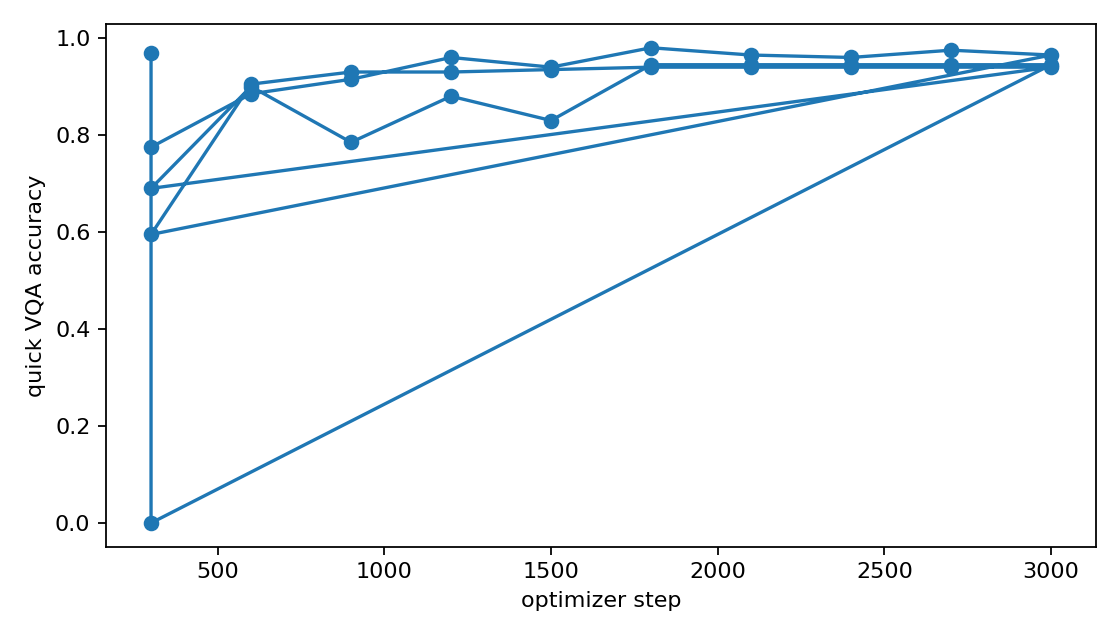
\includegraphics[width=0.7\textwidth]{outputs/partA_phase_vqa_acc.png}
    \caption{Progression of VQA Accuracy across Phase 1, Phase 2, and Phase 3.}
    \label{fig:parta_vqa_acc}
\end{figure}

Simultaneously, we monitored the Forgetting Ratio ($R = PPL_{fine} / PPL_{0}$). As shown in Figure \ref{fig:parta_phase_r}, the utilization of $\lambda = 0.2$ during Phase 2 successfully bounds the forgetting ratio near 1.0. During Phase 3, where $\lambda = 0$, we observe a sharp spike, confirming that without continuous language replay, the LLM rapidly cannibalizes its text priors to optimize visual objectives.

\begin{figure}[H]
    \centering
    \begin{minipage}{0.48\textwidth}
        \centering
        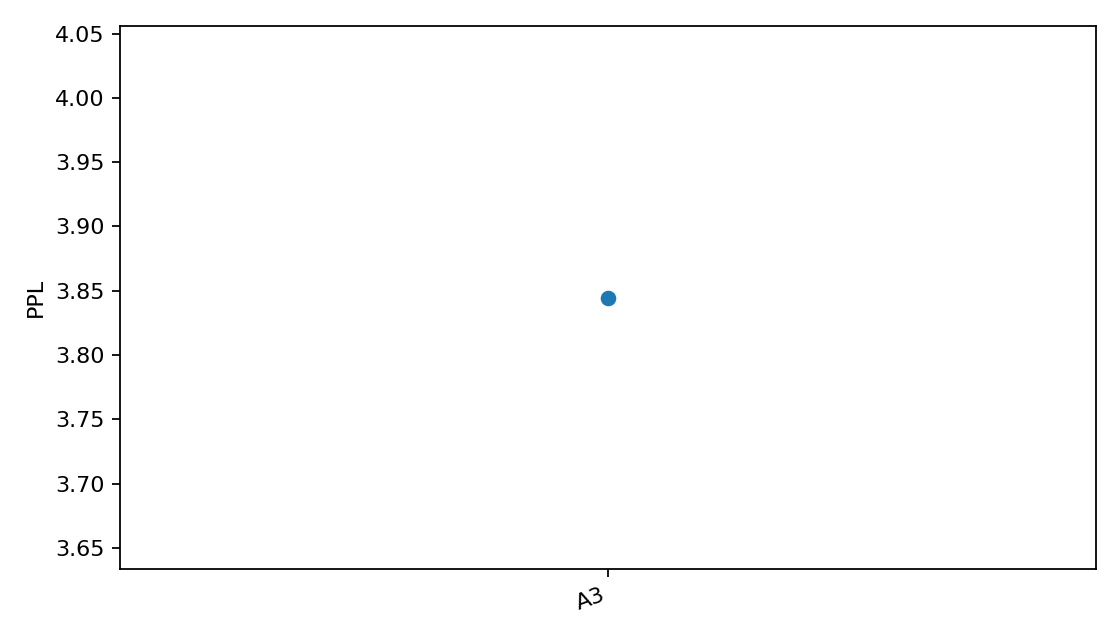
\includegraphics[width=\linewidth]{outputs/partA_phase_ppl.png}
        \caption{Absolute Perplexity of the LLM on the Alpaca evaluation set across training phases.}
        \label{fig:parta_phase_ppl}
    \end{minipage}\hfill
    \begin{minipage}{0.48\textwidth}
        \centering
        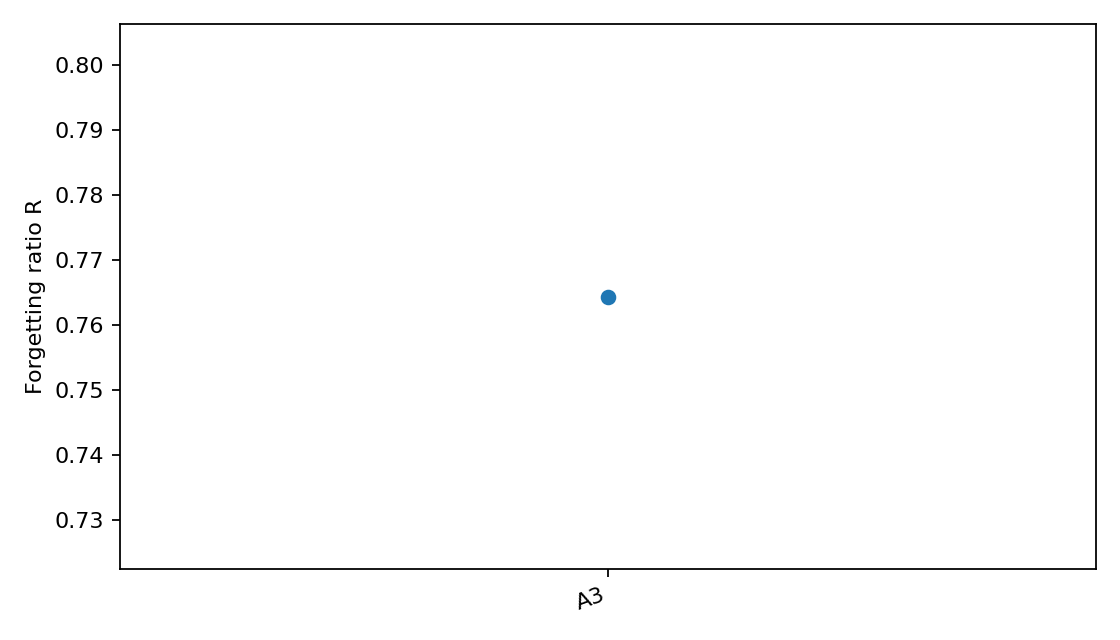
\includegraphics[width=\linewidth]{outputs/partA_phase_R.png}
        \caption{The Forgetting Ratio ($R$). Notice the sharp deviation when replay is disabled in Phase 3.}
        \label{fig:parta_phase_r}
    \end{minipage}
\end{figure}

The final VQA model achieved a \textbf{97.00\% exact-match accuracy}, completely obliterating the majority-class baseline ($34.4\%$) and text-only baseline ($0.0\%$). Qualitative trace failures reveal that errors primarily occur between semantically close natural classes (e.g., misclassifying a low-resolution deer as a frog), verifying that the LLM is genuinely reasoning over the continuous visual embeddings.

\subsubsection{Geometry of the Modality Gap}
A profound question in multimodal alignment is whether the visual and textual embeddings must geometrically intersect. Figure \ref{fig:parta_modality_gap} charts the Modality Gap (the distance between L2-normalized visual and text representations) across training. 

\begin{figure}[H]
    \centering
    \begin{minipage}{0.48\textwidth}
        \centering
        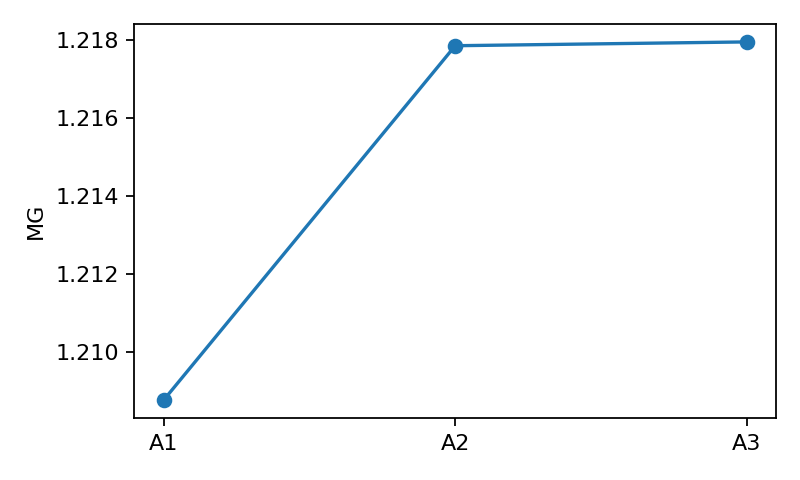
\includegraphics[width=\linewidth]{outputs/partA_modality_gap_phases.png}
        \caption{The Modality Gap remains stubbornly wide ($\approx 1.21$) across all phases.}
        \label{fig:parta_modality_gap}
    \end{minipage}\hfill
    \begin{minipage}{0.48\textwidth}
        \centering
        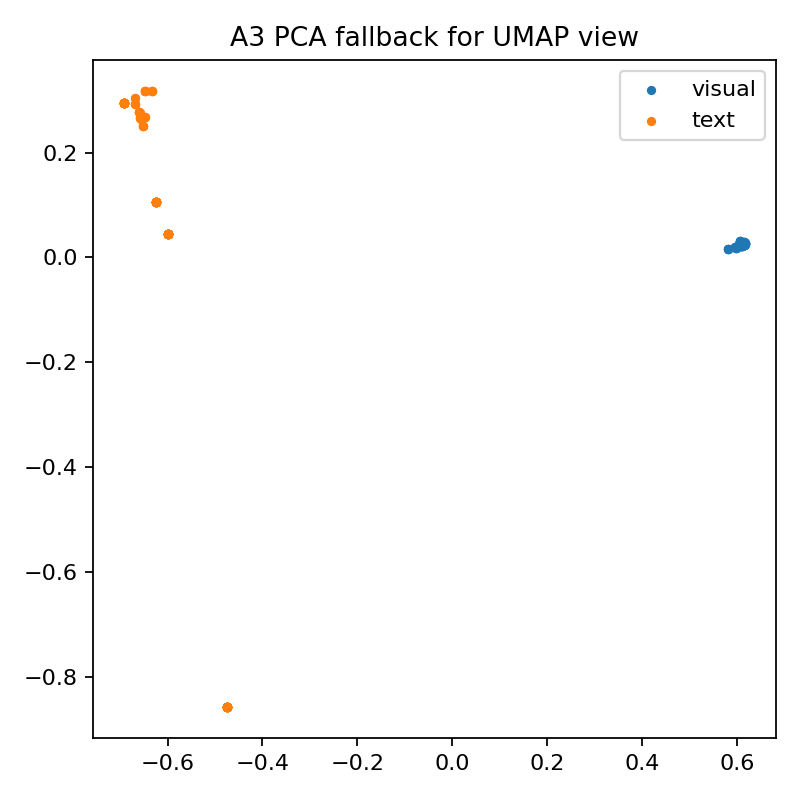
\includegraphics[width=\linewidth]{outputs/partA_modality_umap_or_pca.png}
        \caption{PCA projection clearly visualizing the distinct geometric separation of the visual and text manifolds.}
        \label{fig:parta_umap}
    \end{minipage}
\end{figure}

\textbf{Insight:} The gap remains fixed at $\approx 1.21$ and cross-modal cosine similarity remains practically zero ($\sim 0.007$). Alignment does \textit{not} require closing the geometric gap. The LLM's transformer layers act as sophisticated routers, capable of perfectly mapping isolated visual vectors into correct textual output syntax without forcing geometric overlap.

\section{Part B: Discrete VQ-VAE Tokenization}

Continuous embeddings cannot be autoregressively generated. Part B solves this by training a Vector Quantized Variational Autoencoder (VQ-VAE) to compress images into a discrete 256-token codebook.

\subsection{Methodology and Architecture Setup}

\subsubsection{Synthetic Data and VQ-VAE Regularization}
We procedurally generated a 16x16 geometrical dataset (Figure \ref{fig:synthetic_grid}). The VQ-VAE encoder maps these into a $[4 \times 4 \times 64]$ continuous space, snapped to the nearest discrete codebook vector. To prevent codebook collapse, we implemented Exponential Moving Average (EMA) codebook updates alongside \textit{Dead-Code Restarts}, forcing the model to fully utilize all 256 indices.

\begin{figure}[H]
    \centering
    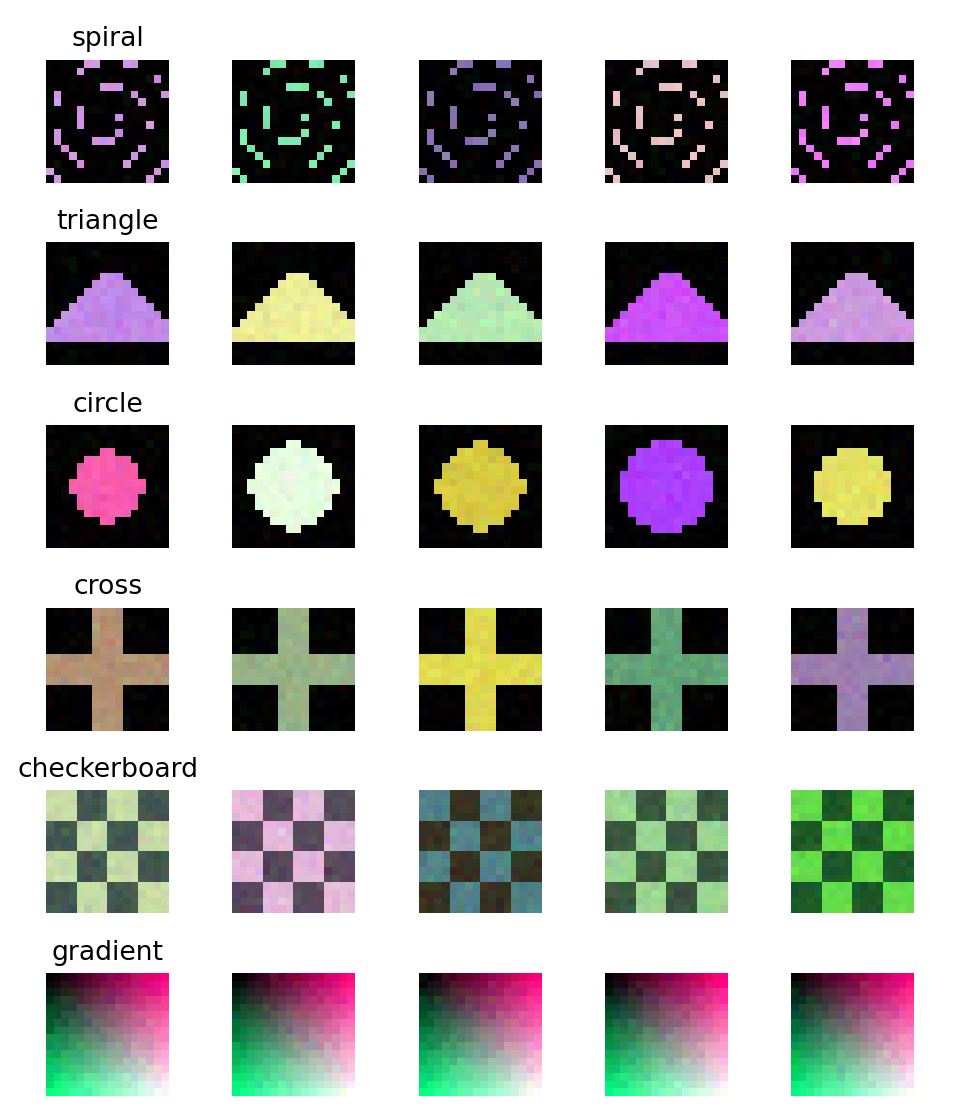
\includegraphics[width=0.6\textwidth]{outputs/synthetic_grid.png}
    \caption{Samples from the procedurally generated geometric dataset utilized for Part B.}
    \label{fig:synthetic_grid}
\end{figure}

\subsubsection{Overlay Embedding and Mixed Optimization}
Expanding the LLM's 49,152 vocabulary introduces millions of untrained parameters. We implemented an \textbf{Overlay Embedding}: a dynamic PyTorch forward hook that routes standard tokens to the frozen text table, and visual IDs to a tiny 258-row overlay table. 
The LLM was optimized using sequential task scheduling to avoid OOM: computing VQA, Image Generation, and Text Replay passes independently before accumulating gradients and stepping the optimizer.

\subsection{Empirical Results and Deep Analysis}

\subsubsection{Symmetric VQA and Logit Separation}
The model achieved a flawless \textbf{1.0000 (100\%)} VQA accuracy on the synthetic dataset, proving the VQ-VAE tokenization successfully retained necessary semantic features. 

To analyze how the LLM delineates visual generation from text generation, we forced autoregressive image generation and examined the logit distribution (Figure \ref{fig:logit_mask}).

\begin{figure}[H]
    \centering
    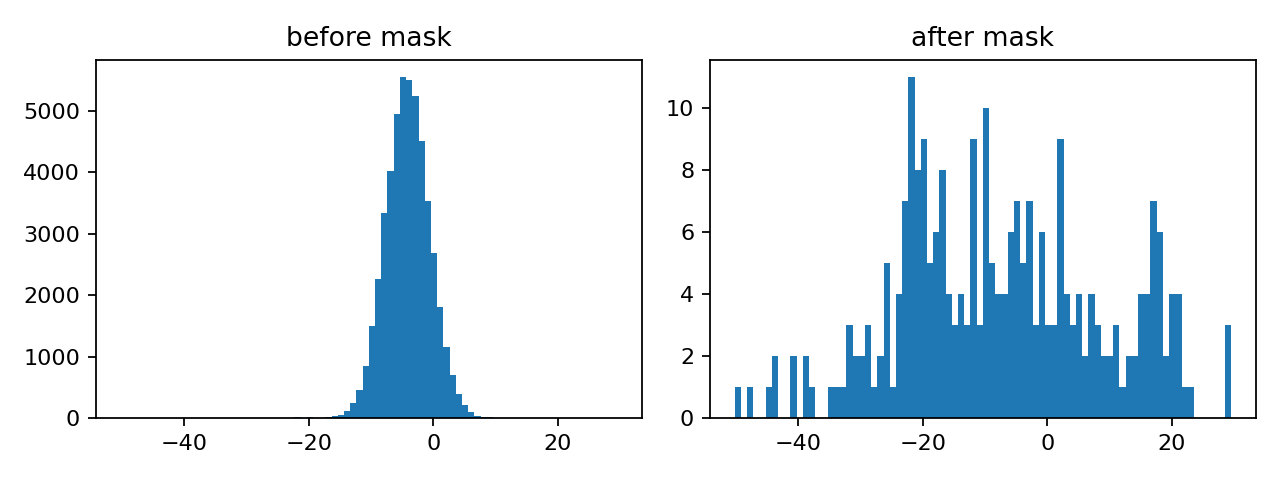
\includegraphics[width=0.6\textwidth]{outputs/partB_logit_mask_hist.png}
    \caption{Logit distribution during image generation. The LLM naturally pushes massive probability mass toward the visual indices, showing semantic delineation between modalities.}
    \label{fig:logit_mask}
\end{figure}

\subsubsection{Autoregressive Generation and Temperature Sweeps}
The unified model successfully acts as a generative visual engine. By sampling 16 autoregressive tokens and decoding them through the frozen VQ-VAE, it synthesized coherent geometry (Figure \ref{fig:generated_grid}). Furthermore, we tested generation stability through a temperature sweep (Figure \ref{fig:temp_sweep}).

\begin{figure}[H]
    \centering
    \begin{minipage}{0.48\textwidth}
        \centering
        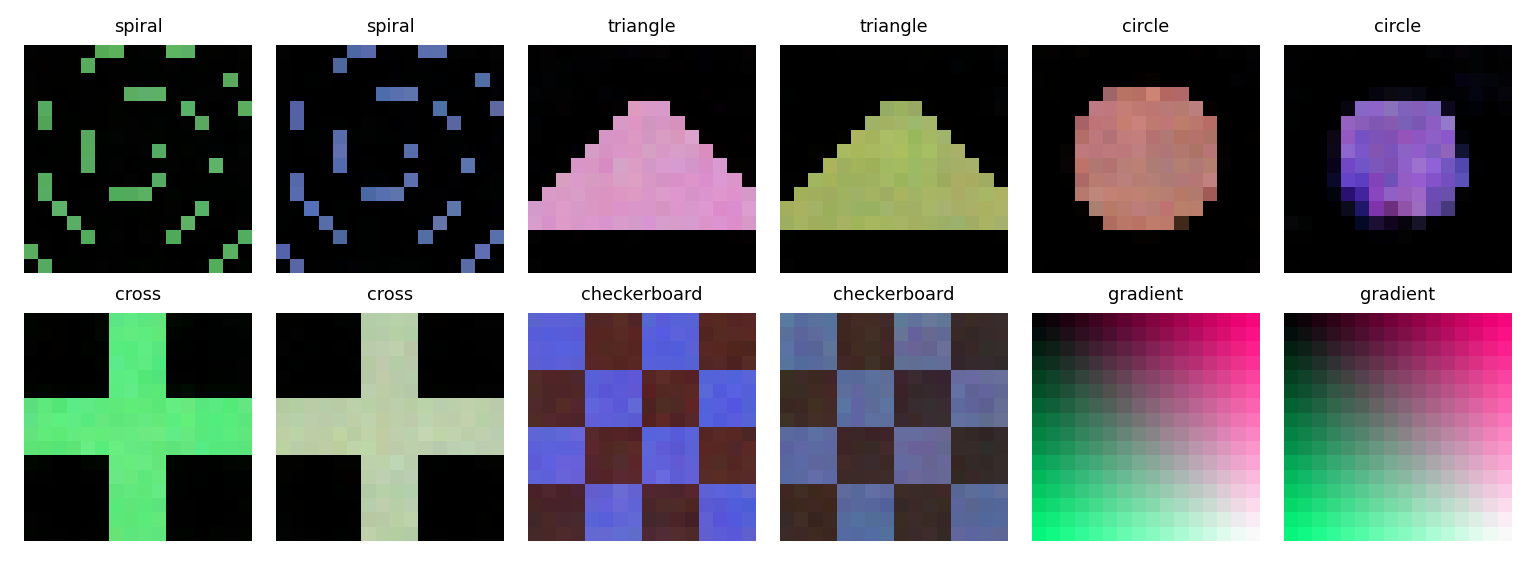
\includegraphics[width=\linewidth]{outputs/partB_generated_grid.png}
        \caption{Autoregressively generated 16x16 geometries decoded from the discrete visual tokens.}
        \label{fig:generated_grid}
    \end{minipage}\hfill
    \begin{minipage}{0.48\textwidth}
        \centering
        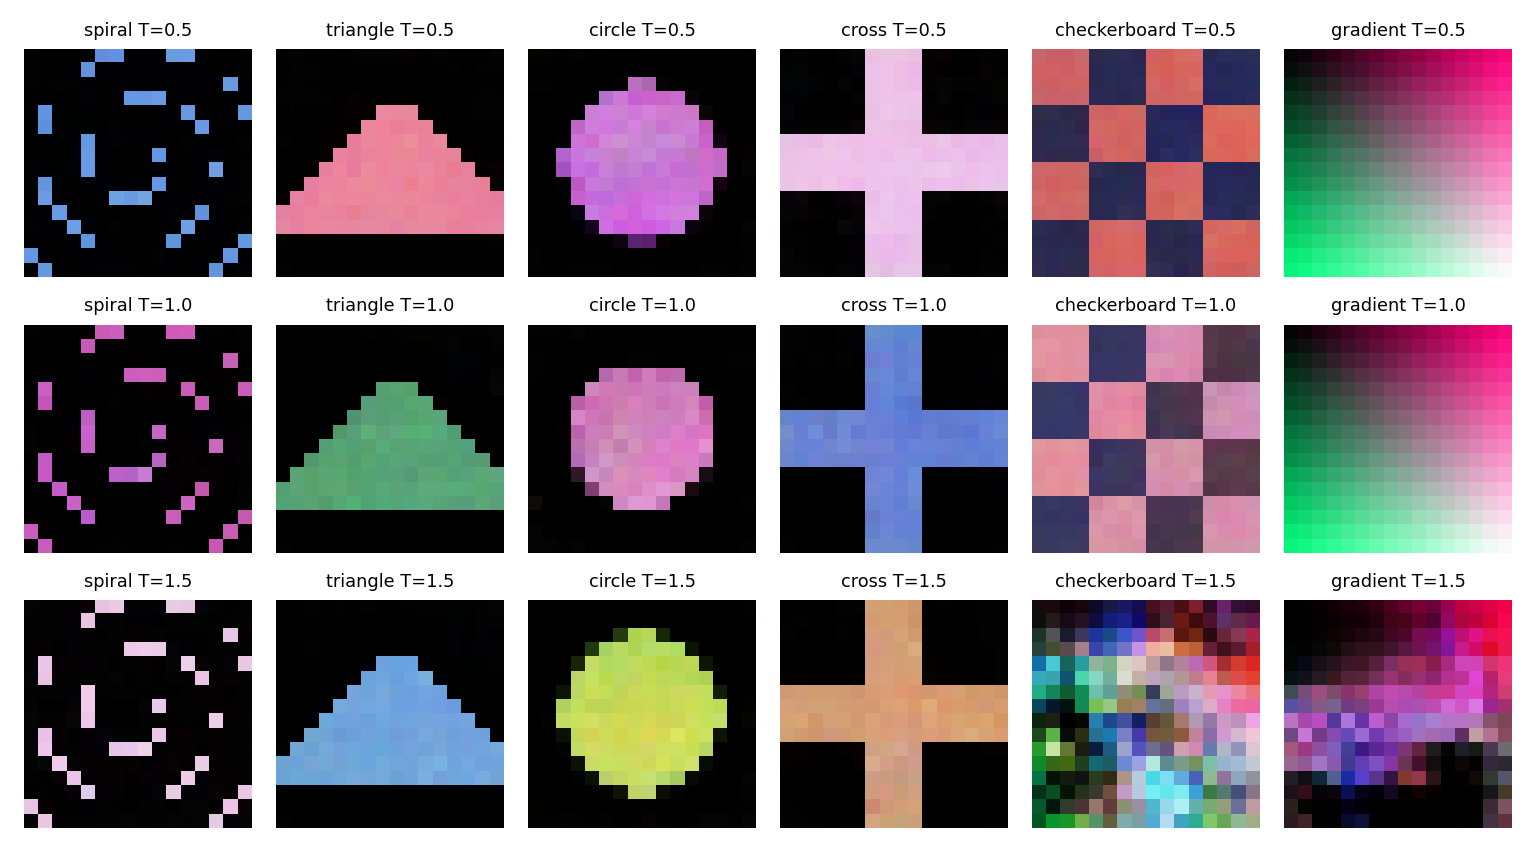
\includegraphics[width=\linewidth]{outputs/partB_temperature_sweep.png}
        \caption{Temperature sweep analysis showing how sampling stochasticity impacts geometric fidelity.}
        \label{fig:temp_sweep}
    \end{minipage}
\end{figure}

\textbf{Insight:} Treating an image as a 1D sequence of 16 tokens inherently destroys vertical spatial coherence, causing occasional row-wrapping artifacts in complex shapes. While discrete tokenization allows the LLM to read and write images symmetrically, this 1D flattening is a fundamental structural limitation compared to 2D diffusion architectures.

\section{Conclusion}

This empirical study demonstrates the successful implementation of two state-of-the-art multimodal paradigms. Continuous connectors efficiently project semantics into language models but leave an unbridgeable generative gap and require strict language replay to prevent catastrophic forgetting. Conversely, Vector Quantized representations solve the generation problem by expanding the language model's native vocabulary, yielding a highly symmetric multimodal engine capable of both complex reasoning and autoregressive visual synthesis. 

\end{document}
